% Tipo de documento. En este caso es un art�culo, para folios A4, tama�o de la fuente 11pt y con p�gina separada para el t�tulo
\documentclass[a4paper,12pt,titlepage]{article}

% Carga de paquetes necesarios. OrdenesArticle es un paquete personalizado
\usepackage[spanish]{babel} 
\usepackage[T1]{fontenc}
\usepackage[ansinew]{inputenx} 
\usepackage[spanish,cap,cont,title,fancy]{OrdenesArticle}
\usepackage{setspace}
\usepackage{array}
\usepackage{graphicx}
\usepackage{hyperref}
\usepackage{pifont}
\usepackage{listings}
\usepackage[usenames,dvipsnames]{color}
\usepackage{colortbl}
\usepackage{makeidx}
\hypersetup{bookmarksopen,bookmarksopenlevel=3,linktocpage,colorlinks,urlcolor=blue,citecolor=blue,
						linkcolor=blue,filecolor=blue,pdfnewwindow,
						pdftitle={Auditor�a a DIGSOL}, 
						pdfauthor={Juan Andrada, Jose Domingo L�pez, Antonio Mart�n Menor, Francisco Jos� Oteo}}


% Macro para definir una lista personalizada 
\newenvironment{milista}%
{\begin{list}{\textbullet}%
{\settowidth{\labelwidth}{\textbullet} \setlength{\leftmargin}{\dimexpr\labelsep+\labelwidth+5pt}
\setlength{\itemsep}{\dimexpr 0.5ex plus 0.25ex minus 0.25ex}
\setlength{\parsep}{\itemsep}
\setlength{\partopsep}{\itemsep}
\addtolength{\topsep}{-7.5pt}
}}%
{\end{list}}

\begin{document}

% En las p�ginas de portada e �ndices, no hay encabezado ni pie de p�gina
\pagestyle{fancy} 

% Se incluye la portada
\begin{titlepage}
	\begin{center}
  	{\LARGE UNIVERSIDAD DE CASTILLA-LA MANCHA} \\
  	\bigskip
  	{\Large ESCUELA SUPERIOR DE INFORM�TICA} \\
  	\vspace{20mm}
  	
\includegraphics[scale=0.45, keepaspectratio]{esi_bw.png} \\
  	\vspace{20mm}
  	{\Huge \textbf{Auditor�a y Seguridad de la Informaci�n}} \\
  	\vspace{10mm}
  	{\LARGE \textsc{\textbf{Auditor�a a DIGSOL}}} \\
  	\vspace{30mm}
  	\today
  	\vspace{30mm}
  	\begin{flushleft}
  		{\large Juan Andrada Romero}\\
  		\vspace{1mm}
  		{\large Jose Domingo L�pez L�pez}\\
  		\vspace{1mm}
  		{\large Antonio Mart�n Menor de Santos}\\
  		\vspace{1mm}
  		{\large Francisco Jos� Oteo Fern�ndez}\\  		
  	\end{flushleft}
	\end{center}
\end{titlepage}

% Se ajusta la separaci�n entre p�rrafos
\parskip=10pt

% Aqui se incluyen los archivos .tex que forman el documento
\section{Carta al Director}
\input{CartaDirector.tex}
\clearpage
\section{Auditor�a}
% -*- coding: utf-8 -*-

\subsection{Problemas relacionados con la Planificaci�n Estrat�gica de TI}

\begin{spacing}{1.4}

% Problemas relacionados con el objetivo de control PO1.1, PO1.2, PO1.4
Consultando al Director General sobre la existencia de un plan estrat�gico de TI, se ha observado que no existe dicho plan. Por tanto, la empresa no est� alineada con las tecnolog�as de la informaci�n, lo que puede suponer, a largo o medio plazo, que la empresa comience a perder presencia en el mercado, ya que para 
seguir siendo competitiva, es necesario investigar nuevas tecnolog�as, actualizar las que ya tiene y aprovechar las oportunidades que ofrece las tecnolog�as de la informaci�n.

Derivado de la inexistencia de un plan estrat�gico de TI que alinee las tecnolog�as con el objetivo de negocio, aparece otro problema, que es la falta de un Departamento de Sistemas de Informaci�n en la organizaci�n de la empresa. Esto provoca que, cuando cada departamento solicita nuevas tecnolog�as, la direcci�n lo aprueba, ya que no hay ning�n especialista que pueda administrar el valor de las TI actuales. Por esta raz�n, la inversi�n en tecnolog�a que realiza la empresa es m�s elevada de lo necesario, lo que puede traducirse en p�rdidas econ�micas importantes a largo plazo. 

% Problemas relacionados con el objetivo de control PO1.6
Por otra parte, como no existe un plan que coordine todo lo relacionado con las tecnolog�as de la informaci�n, no existen portafolios de proyectos que asigne correctamente las prioridades a los diferentes proyectos que maneja la empresa. As�, los desarrolladores inform�ticos (que est�n asociados a los distintos departamentos de la empresa) se limitan a desarrollar las aplicaciones que dichos departamentos necesiten para llevar a cabo su tarea, en el orden en el que se van solicitando. Esto provocar� que no se atiendan a tiempo los proyectos m�s prioritarios para mantener el objetivo de negocio de la empresa y se produzcan p�rdidas econ�micas, adem�s de perder competitividad en el mercado.

\end{spacing}




\clearpage
% -*- coding: utf-8 -*-

\subsection{Problemas relacionados con la Arquitectura de la Informaci�n}

\begin{spacing}{1.4}

%En cuanto a diccionario de datos empresarial y reglas de sintaxis

La empresa DIGSOL carece de un diccionario de datos empresarial que defina las reglas
de sintaxis para los datos de la organizaci�n lo que produce:
-Peor entendimiento entre los usuarios del sistema de TI y del Negocio.
-Posibilidad de creaci�n de elementos de datos incompatibles.

%En cuanto al esquema de clasificacion de datos y la administraci�n de la integridad
Existe un esquema de clasificaci�n de datos definido en el que cada tipo de usuario tiene
acceso a una informaci�n concreta pero al no encriptar la informaci�n que viaja en texto plano
por la red local es f�cilmente interceptable por los dem�s usuarios de la empresa incluso por usuarios
externos ya que adem�s la protecci�n de la wifi se realiza mediante clave WEP que es un tipo de clave 
f�cil de obtener mediante aplicaciones como AirCrack lo que compromete la integridad del sistema.

Los USB y los dispositivos �pticos de los ordenadores de la empresa no 
est�n bloqueados, lo que permitir�a que un usuario malintencionado tomar documentos
 y datos de car�cter confidencial para la empresa, introducir virus o troyanos en el sistema.
%En cuanto a Administraci�n de integridad

No existen procedimientos peri�dicos para cambio de contrase�as de los
usuarios en el sistema. Estas claves son facilitadas en la incorporaci�n del
usuario a la empresa y no son eliminadas tras su despido por el departamento de
SI cuando recibe la confirmaci�n pertinente.

El diagrama de la base de datos es correcto pero su implementaci�n no es coherente con el diagrama dise�ado.
Una vez hemos estudiado la base de datos hemos comprobado que las claves ajenas est�n ausente en la creaci�n 
de las tablas, as� como campos que no deben estar vacios est�n definidos con la posibilidad de serlo.

El acceso a la base de datos es posible si se conoce la cadena de conexi�n a la misma ya que carece de clave de
usuario y de acceso ya que se ha utilizado SQL Server con modo de autenticaci�n de Windows. Es posible obtener 
la ruta de acceso a la base de datos utilizando aplicaciones sniffer que se utilizan para escuchar la 
informaci�n que viaja por nuestra red local de forma que podemos obtener m�s informaci�n de la que el usuario
debiese obtener.

Carece de una base de datos centralizada que contenga la informaci�n completa de la empresa, hay una base de datos
que almacena una parte (productos,empleados,usuarios registrados...) y otra parte que se almacena en ficheros de texto
como facturas... Puesto que las facturas est�n relacionadas con productos, usuarios registrados y empleados entre otros
estas deber�an estar integradas en la base de datos centralizada.



\end{spacing}


\clearpage
La evaluación y gestión de riesgos es un tema que no está abordado de
una forma eficiente en la organización ya que, aunque la empresa
dispone de un plan de riesgos, éste ha sido elaborado por algunos de
los miembros del Consejo de Administración y no existe ningún informe
en el cual se indique quiénes de estos miembros estaban presentes en la
elaboración del plan ni las personas a las que consultaron a la hora
de realizarlo. Además, tampoco existe ningún registro de la técnica de
identificación de riesgos que emplearon (p.e. Delphi) para
seleccionarlos, lo cual puede significar que la elección de éstos
fuese arbitraria o manipulada. En el Anexo ?? se muestra el acta de
los asistentes a dicha reunión. 

Un aspecto a destacar en los riesgos seleccionados y planificados es
que se ciñen al ámbito software dejándo de lado el ámbito hardware, no
teniendo en  cuenta, por ejemplo, factores externos sobre los cuales
la organización puede no tener ningún control debido a su naturaleza
(terremotos, colisiones de aviones, etc...) o incluso el robo de material o
incendios. En el Anexo ?? se puede observar una lista de los riesgos
que deberían ser revisados y/o considerados.

Además, el CIO y el Consejo de Administración han ido elaborando una
lista de los nuevos riesgos que han ido azotando a la organización
pero no los han documentado en términos del impacto que éstos
produjeron ni las estrategias de mitigación o planes de contigencia
que se llevaron a cabo para combatirlos con el objetivo de reutilizarlos
o de mejorarlos. Debido a ésto, algunos riesgos se han producido
en varias ocasiones y no se ha ido reduciendo el impacto. Como prueba
de ello, en el Anexo ?? se puede apreciar que la empresa ha sufrido
dos apagones de luz generales en seis meses, las pérdidas económicas
que supusieron ámbos, el coste de haber desarrollado un plan de
contigencia, y las pérdidas que se habrían producido si dicho plan se
hubiese llevado a cabo.


\clearpage
% -*- coding: utf-8 -*-

\subsection{Problemas relacionados con Adquirir y Mantener Infraestructura Tecnol�gica}

\begin{spacing}{1.4}

% Relacionado con el punto AI3.1
Como ya se ha comentado, la empresa carece de un Departamento de Sistemas de Informaci�n que pueda, entre otras cosas, elaborar un plan para la adquisici�n y mantenimiento de recursos tecnol�gicos. Por ello, cuando cada departamento solicita nuevas tecnolog�as, la direcci�n lo aprueba, ya que no hay ning�n responsable que pueda evaluar si realmente la adquisici�n de hardware es necesaria. Por esta raz�n, la inversi�n en tecnolog�a que realiza la empresa es m�s elevada de lo necesario, lo que puede traducirse en p�rdidas econ�micas importantes a largo plazo. En el Anexo ?? (p�gina \pageref{anexo:facturas}) puede verse un ejemplo de gastos innecesarios en tecnolog�as.

Adem�s, tampoco se realiza un seguimiento ni una evaluaci�n para comprobar que los nuevos recursos obtenidos (principalmete hardware) est�n aportando beneficio a la empresa y est�n ayudando a cumplir su objetivo de negocio. 

\end{spacing}
\clearpage
% -*- coding: utf-8 -*-

\subsection{Problemas relacionados con la adquisici�n de recursos de TI}

\begin{spacing}{1.4}
Al realizar la auditor�a nos hemos fijado en estas �reas dentro de la compa��a: infraestructura hardware, software y la seguridad de los datos.
Respecto a la infraestructura hardware de la empresa, y m�s concretamente, el proceso de adquisici�n de hardware se ha detectado que ni existe ni est� definida una pol�tic a seguir a la hora de adquirir nuevos dispositivos hardware.
Este es, claramente, un riesgo para el TI ya que no se controla qui�n realiza la adquisici�n de hardware, ni si previamente alguien le ha dado una lista de dispositivos que se deben adquirir, etc. No se especif�ca en ning�n documento qui�n es el responsable del desarrollo de unos procedimientos a seguir a la hora de adquirir nuevos dispositivos, existe una lista de proveedores, pero no se ind�ca qui�n estableci� esalista ni qui�n debe actualizarla.
Tampoco se indica si se consulta o no al CEO y al CFO, por lo que existe el riesgo de que cualquier empleado cometa fraudes pudiendo establecer como proveedor a uno con el que haya pactado pero cuyos precios no se ajusten a la pol�tica de gastos o precios de la empresa.
Con respecto a la adquisici�n del software si existen unas pol�ticas definidas. Una vez revisadas se observan algunos riesgos como son la ausencia de un responsable claro que rinda cuentas sobre qu� lista de proveedores se ha hecho y c�mo se mantiene esta (acualiz�ndola a�adiendo o eliminando proveedores).
Una vez que se realiza un pedido, ya sea de hardware o de software, no existe un procedimiento por el que se sigan unas pautas a la hora de realizar pagos o devoluciones; tampoco se indican cl�usulas  u obligaciones que deben cumplirse por parte de los proveedores. Adem�s otro riesgo detectado es que ninguno de los contratos firmados con los proveedores ha sido revisado por un asesor legal.
Al no establecerse esas clausulas contractuales, si un proveedor no satisface un pedido en el periodo acordado puede repercutir en graves p�rdidas econ�micas, debido a que la empresa vende productos por internet y la no disponibilidad de un producto haga que se pierda su venta y que la credibilidad y seriedad de la empresa vea da�ada su imagen.

\end{spacing}
\clearpage
\section{Papeles de Trabajo}
% Los anexos no tienen numeracion de seccion
\titleformat{\subsection}
	{\bfseries\large}
	{}
	{0.5pt}
	{}


\subsection{ANEXO 1: Situaci�n actual de las empresas competidoras} \label{anexo:graficos}

Los gr�ficos de las Figuras \ref{fig:inversion} y \ref{fig:presencia} han sido obtenidos de ?????.

\begin{figure}[!ht]
\centering
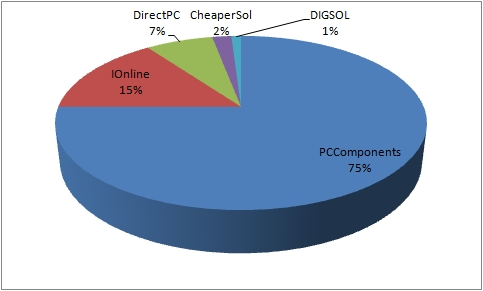
\includegraphics[scale=0.7,keepaspectratio]{./images/investigacion}%
\caption{Porcentaje de inversi�n en investigaci�n de nuevas tecnolog�as}%
\label{fig:inversion}%
\end{figure}

\begin{figure}[!ht]
\centering
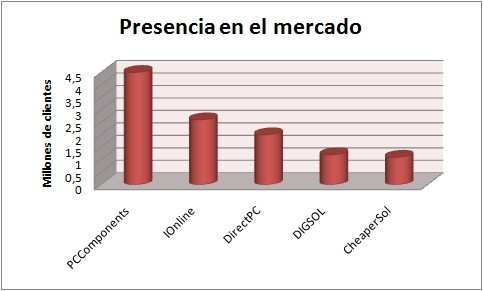
\includegraphics[scale=0.7,keepaspectratio]{./images/presencia}%
\caption{Presencia en el mercado de las empresas}%
\label{fig:presencia}%
\end{figure}

\subsection{ANEXO 2: Organigrama de la empresa DIGSOL} \label{anexo:organigrama}

\begin{spacing}{1.4}
El organigrama mostrado en la Figura \ref{fig:organigrama} ha sido cedido por el Comit� de Direcci�n de la empresa DIGSOL.
\end{spacing}

\begin{figure}[h]
\centering
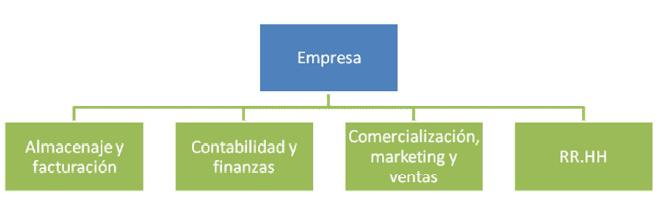
\includegraphics[scale=0.7,keepaspectratio]{./images/organigrama}%
\caption{Organigrama de la empresa DIGSOL}%
\label{fig:organigrama}%
\end{figure}


\subsection{ANEXO 3: Adquisiciones tecnol�gicas} \label{anexo:facturas}

\begin{spacing}{1.4}

Los fragmentos de facturas mostradas en las Figuras \ref{fig:factura} y \ref{fig:facturaAntigua} han sido cedidas por la Direcci�n de la empresa DIGSOL. 

La Figura \ref{fig:facturaAntigua} muestra la adquisici�n que dicha empresa realiz� a mediados del a�o 2008, cuando implant� el servicio de venta Web y actualiz� los equipos de algunos de sus departamentos.

\begin{figure}[ht]
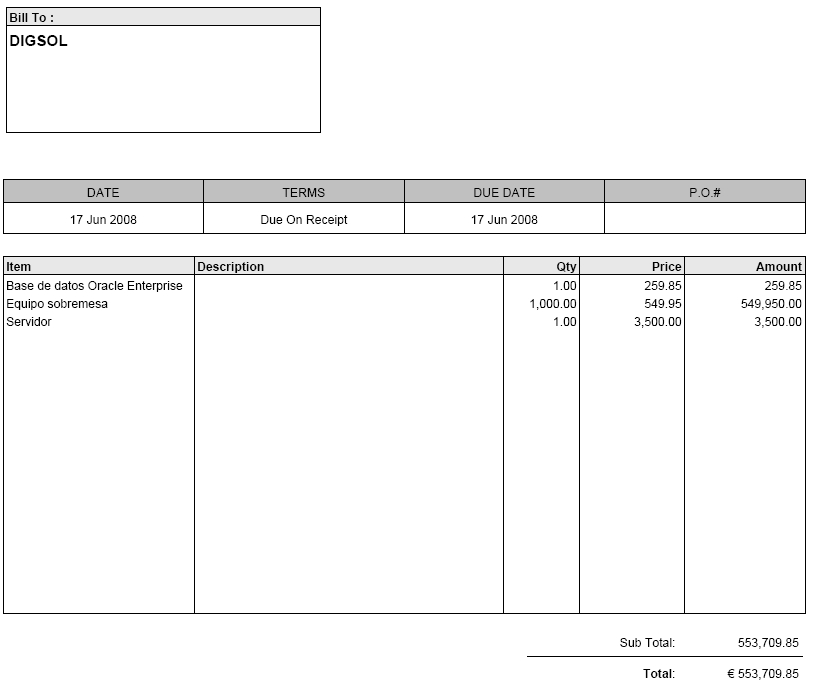
\includegraphics[scale=0.57,keepaspectratio]{./images/facturaAntigua}%
\caption{Fragmento de la factura del 17-Junio-2008}%
\label{fig:facturaAntigua}%
\end{figure}

En la factura de la Figura \ref{fig:factura} se muestra una de las �ltimas adquisiciones que ha realizado la empresa, remarcando gastos que podr�an haberse evitado (en color amarillo) y gastos totalmente innecesarios que no aportan nada de beneficio al negocio (en color rojo). 

\begin{figure}[ht]
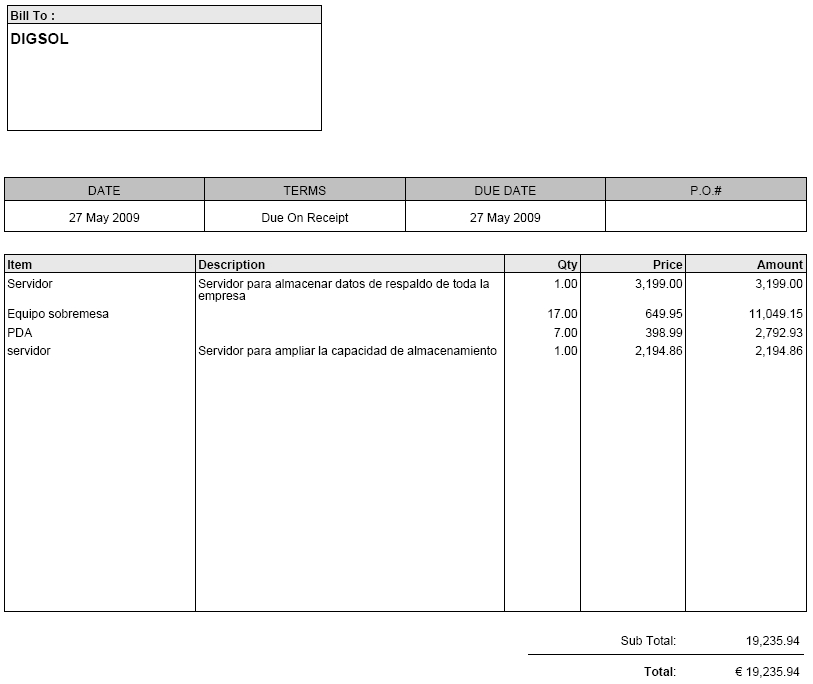
\includegraphics[scale=0.57,keepaspectratio]{./images/factura}%
\caption{Factura del 27-Mayo-2009}%
\label{fig:factura}%
\end{figure}



%El servidor de respaldo es una adquisici�n necesaria, ya que la empresa no lo renovaba desde hace unos 3 o 4 a�os. Sin embargo, la compra de los 17 equipos de sobremesa, destinados al departamento de contabilidad de la sede auditada, es algo innecesario, ya que pr�cticamente la totalidad de equipos se renovaron hace poco m�s de un a�o (coincidiendo con la implantaci�n del sistema Web), tal y como muestra la factura de esa �poca (ver Figura \ref{fig:facturaAntigua}).

%Del mismo modo, adquirir un nuevo servidor para ampliar la capacidad de almacenamiento es, en el momento actual en el que se encuentra la empresa, algo innecsario, pues el servidor que se adquiri� en su dia tiene capacidad suficiente. Podr�a pensarse entonces en qu� es una adquisici�n �til para medio o largo plazo, pero esto no es as�, ya que las tecnolog�as avanzan r�pidamente y en un plazo relativamente corto, existir�n mejores soluciones en el mercado.

%En lo que se refiere a la compra de las PDAs para las personas que integran el comit� de Direcci�n, es un gasto totalmente no justificado e in�til, ya que no se utilizan dichas PDAs para proporcionar valor al negocio. Podr�an aprovecharse para sincronizar los datos de la empresa en las PDAs, atender negocios en ella, etc., pero esto no ocurre as�.


\end{spacing}


\end{document}
